
\documentclass[conference]{IEEEtran}
\usepackage[T1]{fontenc}
\usepackage{amsmath,amssymb}
\usepackage{booktabs,multirow}
\usepackage{graphicx}
\usepackage{array}
\usepackage{tikz}
\usetikzlibrary{positioning,arrows.meta}
\usepackage{xurl}
\usepackage[hidelinks]{hyperref}
\usepackage{balance}

\title{Evaluating Compatibility-Aware Retrieval for Evolving npm APIs: Methodology and Preliminary Retrieval Experiments}

\author{\IEEEauthorblockN{Azmat Ullah}
\IEEEauthorblockA{Research Methodology, FAST-NUCES, Pakistan\\
Registration No.: 26i-7841\\
Email: \texttt{\detokenize{i267841@isb.nu.edu.pk}}}}

\begin{document}
\maketitle

\begin{abstract}
Documentation-augmented code generators may receive API evidence that is relevant to a programming request but incompatible with the library version installed in the target project. This first implementation milestone investigates dependency compatibility as a retrieval constraint for evolving npm packages. We implement a sparse BM25 retriever inspired by the retrieval stage of DocPrompting, an offline dense latent-semantic-analysis (LSA) retriever, a lockfile-first package-version resolver, and a conservative compatibility gate that requires an explicitly annotated valid target version. We construct a controlled pilot from 18 changes described in official Express, Mongoose, and React Router migration guides, with 36 version-conditioned tasks and 36 author-written document paraphrases. On these tasks, correct-document Top-1 accuracy is 47.2\% for BM25 and 41.7\% for LSA. Adding the compatibility gate improves the respective rates to 80.6\% and 77.8\%, while first-ranked compatibility increases from 50.0\% to 100.0\% in both settings. These numbers measure retrieval rather than executable code generation. The dataset is small, manually labeled, and constructed to contain version conflicts; therefore, the reported gains do not establish general effectiveness over existing version-aware tools. We reimplement a component of the published DocPrompting approach but do not reproduce that paper's original benchmark results. A separate Node.js script is prepared for genuine pinned-package API probes, but those probes have not been run because package downloads are unavailable in the experiment environment. These preliminary experiments establish a reproducible starting point for later baseline reproduction and execution-based evaluation.
\par\noindent Code repository: \url{https://github.com/azmatullah93/npm-compatibility-aware-rag}
\end{abstract}

\begin{IEEEkeywords}
code retrieval, API evolution, version compatibility, BM25, npm
\end{IEEEkeywords}

\section{Introduction}
Large language models can generate source code with help from library documentation. The external information matters because APIs continue to change after a model has been trained. DocPrompting showed how retrieving documentation before generation can improve code generation \cite{docprompting}. CodeRAG-Bench subsequently found that useful retrieved context can help, but that retrieving and using such context reliably remains difficult \cite{coderag}.

The difficulty considered here is narrower than ordinary document relevance. Documentation for an older version of a library can describe the same task as documentation for the installed version, but its API signature or behavior may differ. LibEvolutionEval showed that code generation can change noticeably across library versions \cite{libevolution}. GitChameleon 2.0 evaluated executable version-specific Python tasks and found continued difficulty for current code-generation approaches \cite{gitchameleon}. In the npm ecosystem, a large empirical study found many documented JavaScript and TypeScript breaking changes \cite{npmchanges}.

The general RAG literature also challenges the assumption that a relevant document must be safe to use. Hong and colleagues examined retrieved documents containing relevant but conflicting evidence and found that they can mislead model outputs \cite{gullible}. In programming tasks, conflicting evidence can be tied to actual package versions rather than only to conflicting natural-language facts.

Our research therefore asks whether the retrieval stage should explicitly account for the target project's installed dependency version. This first milestone contributes (i) a reproducible controlled collection of API-version retrieval cases, (ii) a reimplementation of a DocPrompting-style sparse BM25 retriever, (iii) an additional dense LSA retrieval baseline, (iv) a lockfile-based compatibility gate, and (v) four-method retrieval measurements. The method's impact on generated code and its behavior on larger real documentation collections remain open. Section II reviews relevant work; Section III specifies the dataset and method; Section IV reports the pilot results and remaining reproduction work; Section V concludes.

\subsection{Research Questions and Objectives}
The full study follows three linked questions. \textit{RQ1} asks how increasing the proportion of semantically relevant but version-incompatible API documentation changes executable code correctness; objective \textit{O1} is to measure that effect under controlled evidence conflict. \textit{RQ2} asks whether explicit dependency compatibility improves the selection of valid documentation; \textit{O2} is to implement and compare compatibility-constrained retrieval with ordinary retrieval. \textit{RQ3} asks whether improvements in document retrieval translate into executable code under fixed target library versions; \textit{O3} is to conduct end-to-end code generation and execution comparisons. The present milestone directly evaluates only the \emph{retrieval-stage portion of RQ2}. RQ1 and RQ3 require subsequent controlled document-injection and real npm code-execution experiments.

\section{Related Work}
\subsection{Documentation-Assisted Code Generation}
DocPrompting retrieves API documentation with sparse or dense retrieval and conditions a code generator on the selected evidence \cite{docprompting}. Its published experiments use the CoNaLa and tldr benchmarks and several generator architectures. The present work reimplements only the BM25-style sparse retrieval principle on a different corpus, not the original Elasticsearch-based retrieval deployment, trained generator, or original benchmark. A separate TF-IDF/SVD model supplies a dense non-neural comparison. CodeRAG-Bench compares retrievers and language models across multiple code-generation settings and shows that retriever quality is a substantial bottleneck \cite{coderag}. Both studies motivate separating retrieval accuracy from generation correctness.

\subsection{Version-Conditioned Generation and npm Evolution}
LibEvolutionEval studies public Python libraries as APIs change and evaluates version-specific documentation retrieval \cite{libevolution}. GitChameleon 2.0 adds 328 executable version-conditioned problems across 26 Python libraries \cite{gitchameleon}. These publications show that version-specific generation is already an established research problem. Our proposed extension isolates conflicting same-API versions at the retrieval stage, with npm as the experimental domain. The npm breaking-change study by Kong and colleagues establishes that syntactic and behavioral library changes are common enough to make this a practical problem \cite{npmchanges}.

\subsection{Conflicting Retrieved Evidence}
Hong and colleagues showed that even query-relevant documents can introduce harmful counterfactual conflicts in RAG \cite{gullible}. In our setting, a document is potentially misleading if it prescribes API usage that does not apply to the package version installed in the target project. Unlike a general QA conflict, this compatibility question can eventually be evaluated by executing generated code with the required dependency.

\begin{table}[t]
\centering
\caption{Critical comparison of closely related approaches}
\label{tab:related}
\setlength{\tabcolsep}{2.7pt}
\begin{tabular}{p{0.24\columnwidth}p{0.31\columnwidth}p{0.34\columnwidth}}
\toprule
Study & Main contribution & Limitation for this study\\
\midrule
DocPrompting \cite{docprompting} & Retrieves docs before generation & No explicit mixed-version npm conflict setting\\
CodeRAG-Bench \cite{coderag} & Broad code RAG evaluation & Retrieval utility not identical to API-version validity\\
LibEvolutionEval \cite{libevolution} & Version-specific generation & Investigates Python libraries\\
GitChameleon 2.0 \cite{gitchameleon} & Executable version tests & Focuses on Python tasks, not npm retrieval conflicts\\
Why So Gullible? \cite{gullible} & Counterfactual RAG noise & Not executable package-version compatibility\\
\bottomrule
\end{tabular}
\end{table}

\section{Materials and Methods}

\subsection{Dataset Construction}
We prepared a pilot corpus using official migration guides for Express 4 to 5, Mongoose 6 to 7, and React Router 5 to 6 \cite{express,mongoose,router}. We selected six distinct changes per library and wrote two short documentation \emph{paraphrases} for each change, one representing each tested historical version. Each migration yields two retrieval tasks with the same natural-language intent but different target versions, giving 18 migrations, 36 tasks, and 36 documents. These are author-written research fixtures, not automatically collected official documentation chunks.

\begin{table}[t]
\centering
\caption{Composition of the controlled pilot dataset}
\label{tab:data}
\begin{tabular}{lrrr}
\toprule
Library & Migrations & Tasks & Documents\\
\midrule
Express 4/5 & 6 & 12 & 12\\
Mongoose 6/7 & 6 & 12 & 12\\
React Router 5/6 & 6 & 12 & 12\\
\midrule
Total & 18 & 36 & 36\\
\bottomrule
\end{tabular}
\end{table}

Representative changes include Express wildcard routing, removal of Mongoose query callbacks, and the React Router transition from \texttt{useHistory} to \texttt{useNavigate}. Each document stores \texttt{package}, \texttt{api\_id}, \texttt{version}, an explicit set of valid versions, a paraphrased API description, and a source URL. Each task stores its query, exact target version, package metadata, and a manually designated correct document. Data preparation consists of manually isolating the migration operation, rewriting a short guidance sentence for each version, and assigning a version label and source URL. We did not scrape or split long official documentation pages. Labels were checked against the migration-guide descriptions but not independently double-annotated. No training or validation partition is used because the pilot introduces no trained neural model; LSA is fitted to the complete unlabeled document corpus. The same task set is then used for descriptive method comparison, not as a held-out test set for a tuned production system. A later study must use independent annotations, larger held-out data, and genuine archived documentation.

\subsection{Problem Formulation}
Let $q$ be a programming request, $p$ a package, $v$ the installed version, and $D_p$ the available documents associated with that package. We seek the document $d^*$ describing the requested operation and compatible with $v$. A conventional sparse retrieval baseline ranks by:
\begin{equation}
d^*_{\mathrm{BM25}}=\arg\max_{d\in D_p} s_{\mathrm{BM25}}(q,d).
\end{equation}
For BM25, with query terms $t$, term frequency $f(t,d)$, document length $|d|$, and average length $\overline{\ell}$,
\begin{equation}
s_{\mathrm{BM25}}(q,d)=\sum_{t\in q}\mathrm{IDF}(t)
\frac{f(t,d)(k_1+1)}
{f(t,d)+k_1(1-b+b|d|/\overline{\ell})}.
\end{equation}
Our implementation uses $k_1=1.5$ and $b=0.75$. The sparse-retrieval principle is adapted from DocPrompting \cite{docprompting}; these local implementation choices are not claimed to reproduce the original Elasticsearch ranking scores.

As a second retrieval baseline, we use latent semantic analysis (LSA). A word-unigram/bigram TF-IDF matrix $X$ is reduced using truncated singular-value decomposition $X \approx U_k\Sigma_k V_k^\top$, with $k=16$ and random seed 0. Each document and query is projected into the same dense space and ranked by normalized dot product:
\begin{equation}
s_{\mathrm{LSA}}(q,d)=\frac{\mathbf z_q^{\top}\mathbf z_d}{\|\mathbf z_q\|_2\|\mathbf z_d\|_2}.
\end{equation}
This is a conventional corpus-fitted, dense latent-semantic baseline, not a pretrained transformer embedding model. The gate below is applied identically to BM25 and LSA.

Each pilot document has an explicitly annotated validity set $V(d)$. We define:
\begin{equation}
C(d,v)=\begin{cases}1,&v\in V(d),\\0,&\text{otherwise}.\end{cases}
\end{equation}
The compatibility-aware retrieval score is:
\begin{equation}
s_{\mathrm{gate}}(q,d,v)=
\begin{cases}
s_{\mathrm{base}}(q,d),&C(d,v)=1,\\
-\infty,&C(d,v)=0.
\end{cases}
\end{equation}
The method reranks only compatible candidates. If no compatible document is available, it abstains instead of silently returning an incompatible document. This is a conservative first-stage component and not yet an automatic method for inferring validity across undocumented releases.

\subsection{Workflow and Implementation}
\begin{figure*}[t]
\centering
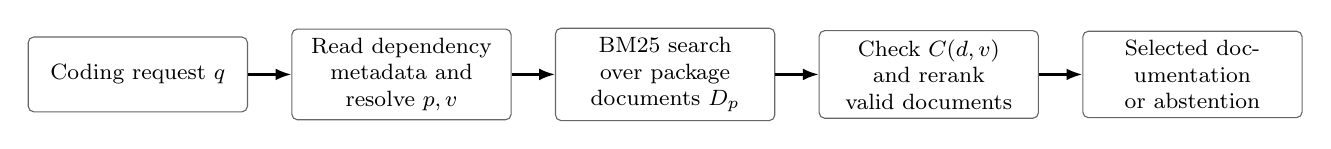
\begin{tikzpicture}[
node distance=0.5cm and 0.55cm,
blk/.style={draw=black!60,rounded corners=2pt,minimum height=0.95cm,text width=2.55cm,align=center,font=\footnotesize},
arr/.style={-{Latex[length=2mm]},thick}
]
\node[blk] (req) {Coding request $q$};
\node[blk,right=of req] (meta) {Read dependency metadata and resolve $p,v$};
\node[blk,right=of meta] (ret) {BM25 search over package documents $D_p$};
\node[blk,right=of ret] (gate) {Check $C(d,v)$ and rerank valid documents};
\node[blk,right=of gate] (out) {Selected documentation or abstention};
\draw[arr] (req)--(meta);
\draw[arr] (meta)--(ret);
\draw[arr] (ret)--(gate);
\draw[arr] (gate)--(out);
\end{tikzpicture}
\caption{Implemented retrieval-stage workflow. LLM generation and real npm execution are not yet part of this pilot.}
\label{fig:workflow}
\end{figure*}

The retrieval prototype is implemented in Python without external model downloads. It uses the standard library for BM25 and scikit-learn for offline LSA vectors. It parses \texttt{package.json} and prefers the resolved exact version from \texttt{package-lock.json}. If only a caret or tilde range is available and there is no lockfile, the resolver rejects the ambiguous input rather than guessing. After identifying the package and target version, it performs either BM25 or LSA retrieval using the same package-level candidate restriction for all four conditions. The compatibility-aware condition then drops all documents not explicitly labeled valid for the resolved version. The prototype uses exact listed validity labels; it does not infer semantic compatibility from a major-version number. Ten unit tests check dataset integrity, lockfile priority, rejection of unresolved version ranges, LSA ranking, compatibility exclusion, and safe abstention. The JavaScript probe script uses 	exttt{npm install} in isolated temporary directories to run specific Express and Mongoose API checks; that script is not part of the measured pilot and remains unexecuted until the packages can be downloaded.

\section{Experimental Results and Discussion}

\subsection{Experimental Setup}
Retrieval experiments were run in a Linux x86-64 environment with Python 3.13.5, scikit-learn 1.8.0, and NumPy 2.3.5. No GPU, hosted LLM API, or network-dependent inference was used. All four conditions use the same 36 manually constructed tasks and the same 36-document corpus. Package-level candidate restriction is applied equally. Both retrieval baselines are deterministic with fixed settings, and the same document-ID tie-breaking rule is used across conditions. LSA uses 16 components and random seed 0. BM25 uses $k_1=1.5$ and $b=0.75$. Evaluation measures the rank of an annotated correct document and whether the first retrieved item is labeled compatible with the target package version. The system does \emph{not} execute generated JavaScript code, so it cannot yet estimate Pass@1 or the frequency of actual runtime failures.

\subsection{Evaluation Metrics}
For $N$ tasks with top-ranked document $r_i$ and annotated correct document $g_i$, correct-document Top-1 accuracy is:
\begin{equation}
\mathrm{Top1}=\frac{1}{N}\sum_{i=1}^{N}\mathbb{I}(r_i=g_i).
\end{equation}
Compatibility@1 replaces the equality test with $\mathbb{I}(C(r_i,v_i)=1)$. Recall@3 is the fraction of tasks whose annotated correct document occurs in the top three results; MRR@3 averages the reciprocal rank of that correct document, using zero if absent. These retrieval metrics directly assess the proposed retrieval-stage gap. Execution-based metrics are reserved for later experiments.

\subsection{Baseline Implementation and Reproduction Status}
The principal reference paper is DocPrompting (ICLR 2023) \cite{docprompting}. Its published abstract reports absolute gains of 2.85 percentage points in Pass@1 and 4.39 points in Pass@10 for one Python CoNaLa setting, as well as improvements on Bash tldr. We reimplemented a BM25-based documentation retrieval stage and evaluated it on a different, controlled npm dataset. This is a \emph{partial component reimplementation}, not a faithful result reproduction. The paper's reported CodeT5 pass@1/pass@10 and Bash exact-match improvements are produced with different original datasets, retriever and generator configurations. We did not download those original checkpoints, train the original models, run CoNaLa or tldr, or reproduce the published numerical scores. A complete baseline reproduction remains required before the final assignment. The difference in dataset, retrieval engine, and absence of a generator makes direct numerical comparison with the original paper invalid.

\subsection{Preliminary Retrieval Results}
\begin{table}[t]
\centering
\caption{Observed retrieval metrics (36 manually curated tasks)}
\label{tab:results}
\setlength{\tabcolsep}{3pt}
\begin{tabular}{lrrrr}
\toprule
Method & Top-1 & Comp.@1 & R@3 & MRR@3\\
\midrule
BM25 & 47.2\% & 50.0\% & 83.3\% & 0.648\\
BM25 + version & 80.6\% & 100\% & 100\% & 0.884\\
LSA & 41.7\% & 50.0\% & 83.3\% & 0.611\\
LSA + version & 77.8\% & 100\% & 100\% & 0.875\\
\bottomrule
\end{tabular}
\end{table}

Adding the explicit version constraint increases correct-document Top-1 by 33.4 percentage points for BM25 (17/36 to 29/36) and 36.1 points for LSA (15/36 to 28/36). The number of top-ranked version-compatible documents rises from 18/36 to 36/36 for either retriever. This second outcome is largely expected because the method filters directly against manually supplied validity labels; it is a function test rather than independent evidence of inferred compatibility. Correct-document Top-1 is below 100\% because version checking cannot always select the correct API among different valid documents for the same package.

\begin{figure}[t]
\centering
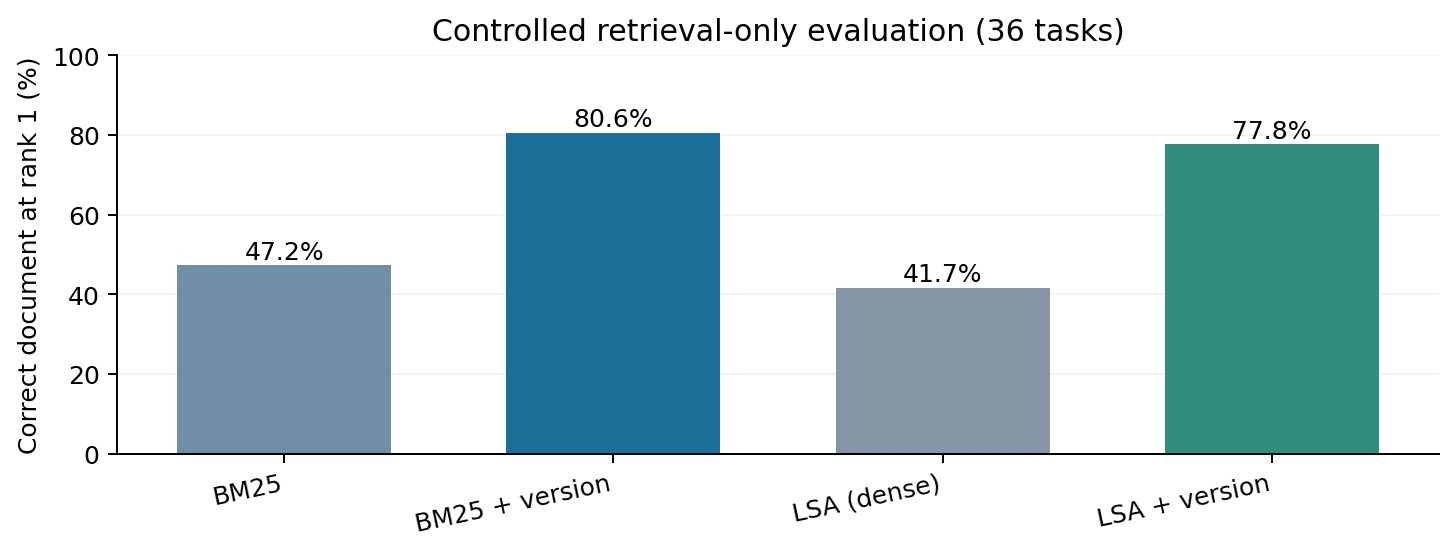
\includegraphics[width=\columnwidth]{../outputs/retrieval_four_methods.png}
\caption{Measured correct-document Top-1 retrieval accuracy; not generated-code execution accuracy.}
\label{fig:retrieval}
\end{figure}

\begin{table}[t]
\centering
\caption{Correct-document Top-1 hits per npm library (12 tasks each)}
\label{tab:package}
\setlength{\tabcolsep}{3pt}
\begin{tabular}{lrrrr}
\toprule
Package & BM25 & BM25+V & LSA & LSA+V\\
\midrule
Express & 6 & 11 & 5 & 9\\
Mongoose & 5 & 9 & 5 & 9\\
React Router & 6 & 9 & 5 & 10\\
\bottomrule
\end{tabular}
\end{table}

These per-package outcomes show that retrieval limitations remain even after known incompatible documents are excluded. For example, the BM25 + version gate still misses 3 of the 12 React Router task-specific gold documents because other version-valid items can have higher lexical scores. Both retrievers score the same textual requests for the old and new target versions, so changes in output after gating come from the target version metadata and not from changes to the query.

\subsection{Ablation, Prepared npm Probes, and Threats to Validity}
Removing the compatibility gate is the ablation of its contribution for each of the BM25 and LSA retrievers. This identifies the effect of a simple preannotated validity filter, but \emph{does not} show that a new compatibility-inference algorithm exceeds existing metadata filters. The corpus contains paired, author-written descriptions selected around documented breaking changes, making relevance ranking and version filtering more controlled than deployment. The same author prepared and labeled the corpus. Tasks are paired by migration, so the 36 observations are not independent samples for formal generalization testing.

An \texttt{execution/npm\_version\_probes.cjs} script is included to install Express 4 and 5 and Mongoose 6 and 7 into separate temporary projects and check a small set of version-dependent APIs. Its JavaScript syntax has been verified using Node.js 22.16.0. \emph{No actual package installation or API-probe results are claimed here}: npm network access was not available during this milestone. It must also be emphasized that these probes assess author-specified API examples, not LLM-generated outputs. Therefore, Pass@1 for LLM generation, generalization across unseen package changes, runtime-error-rate reduction, and published DocPrompting result reproduction are not established by the present experiments.

The next experiments should use a larger corpus of authentic versioned documentation, independently verified annotations, real pinned-library execution tests, a pretrained neural dense retriever, actual LLM-generated solutions, and fair comparison against exact metadata filtering. The published DocPrompting benchmark should be reproduced on its original data and model configurations before reporting a paper-level baseline reproduction. Statistical comparisons should account for paired tasks and report uncertainty intervals.

\section{Conclusion and Future Work}
This milestone implemented two documentation retrievers and a dependency-version compatibility gate, and evaluated four retrieval conditions on 36 controlled API retrieval tasks. On these tasks, explicit version checking removed incompatible top-ranked documents and raised BM25 correct-document retrieval from 47.2\% to 80.6\% and LSA correct-document retrieval from 41.7\% to 77.8\%. The result demonstrates that the prototype works on its own curated test cases; it does not yet show improved LLM code generation or a general advantage over established metadata filtering methods. The full research will require faithful baseline reproduction, real npm execution, stronger compatibility reasoning, independent dataset validation, and evaluation across a broader set of libraries. The prototype and dataset are intended to serve as the starting point for that work.

\balance
\begin{thebibliography}{99}
\bibitem{docprompting}
S. Zhou, U. Alon, F. F. Xu, Z. Wang, Z. Jiang, and G. Neubig, ``DocPrompting: Generating Code by Retrieving the Docs,'' in \emph{Proc. Int. Conf. Learn. Representations (ICLR)}, 2023. [Online]. Available: \url{https://openreview.net/forum?id=ZTCxT2t2Ru}.

\bibitem{coderag}
Z. Z. Wang, A. Asai, X. V. Yu, F. F. Xu, Y. Xie, G. Neubig, and D. Fried, ``CodeRAG-Bench: Can Retrieval Augment Code Generation?,'' in \emph{Findings Assoc. Comput. Linguistics: NAACL}, 2025, pp. 3199--3214, doi: 10.18653/v1/2025.findings-naacl.176.

\bibitem{libevolution}
S. Kuhar, W. U. Ahmad, Z. Wang, N. Jain, H. Qian, B. Ray, M. K. Ramanathan, X. Ma, and A. Deoras, ``LibEvolutionEval: A Benchmark and Study for Version-Specific Code Generation,'' in \emph{Proc. NAACL}, 2025, pp. 6826--6840, doi: 10.18653/v1/2025.naacl-long.348.

\bibitem{gitchameleon}
D. Misra, N. Islah, V. May, B. Rauby, Z. Wang, J. Gehring, A. Orvieto, M. S. Chaudhary, E. B. Muller, I. Rish, S. E. Kahou, and M. Caccia, ``GitChameleon 2.0: Evaluating AI Code Generation Against Python Library Version Incompatibilities,'' in \emph{Proc. ACL}, 2026, pp. 46792--46831, doi: 10.18653/v1/2026.acl-long.2170.

\bibitem{npmchanges}
D. Kong, J. Liu, L. Bao, and D. Lo, ``Toward Better Comprehension of Breaking Changes in the NPM Ecosystem,'' \emph{ACM Trans. Softw. Eng. Methodol.}, vol. 34, no. 4, Art. no. 111, pp. 1--23, 2025, doi: 10.1145/3702991.

\bibitem{gullible}
G. Hong, J. Kim, J. Kang, S.-H. Myaeng, and J. J. Whang, ``Why So Gullible? Enhancing the Robustness of Retrieval-Augmented Models against Counterfactual Noise,'' in \emph{Findings Assoc. Comput. Linguistics: NAACL}, 2024, pp. 2474--2495, doi: 10.18653/v1/2024.findings-naacl.159.

\bibitem{express}
Express.js, ``Upgrading to Express 5,'' [Online]. Available: \url{https://expressjs.com/en/guide/migrating-5/}. Accessed: Nov. 8, 2026.

\bibitem{mongoose}
Mongoose, ``Migrating from 6.x to 7.x,'' [Online]. Available: \url{https://mongoosejs.com/docs/7.x/docs/migrating_to_7.html}. Accessed: Nov. 8, 2026.

\bibitem{router}
React Router, ``Upgrading from v5,'' [Online]. Available: \url{https://reactrouter.com/docs/en/v6/upgrading/v5}. Accessed: Nov. 8, 2026.

\end{thebibliography}
\end{document}
